\documentclass[a4paper, oneside, 12pt]{book}
\usepackage[italian]{babel}
\usepackage[T1]{fontenc}
\usepackage{hyperref}
\usepackage{graphicx}
\usepackage[dvipsnames]{xcolor}
\usepackage{geometry}
\usepackage{float}
% \geometry{
% a4paper,
% margin=1in,
%total={6in,8in},
%left=20mm,
%top=0mm,
% }


\begin{document}
\pagenumbering{arabic}

\frontmatter

\title{Progetto ingegneria del software \\ "Lavoratori stagionali"}
\author{Enrico Bragastini \\ Davide Bianchini \\ Andrea Mafficini}
% \date{}
\maketitle

\tableofcontents

\chapter{Specifiche dei casi d'uso}

\section{Note generali}
% \subsection{Note generali} 
Si vuole progettare un sistema informatico di una agenzia che fornisce servizi di supporto alla ricerca
di lavoro stagionale. I lavoratori interessati possono iscriversi al servizio, rivolgendosi agli sportelli
dell’agenzia. Il sistema deve permettere la gestione delle anagrafiche e la ricerca di lavoratori
stagionali, nei settori dell’agricoltura e del turismo.
I responsabili del servizio, dipendenti dell’agenzia, inseriscono i dati dei lavoratori. Per ogni
lavoratore vengono memorizzati i dati anagrafici (nome, cognome, luogo e data di nascita,
nazionalità), indirizzo, recapito telefonico personale (se presente), email, le eventuali
specializzazioni/esperienze precedenti (bagnino, barman, istruttore di nuoto, viticultore,
floricultore), lingue parlate, il tipo di patente di guida e se automunito. Sono inoltre memorizzati i
periodi e le zone (comuni), per i quali il lavoratore è disponibile. Di ogni lavoratore si memorizzano
anche le informazioni di almeno una persona da avvisare in caso di urgenza: nome, cognome,
telefono, indirizzo email.
I dipendenti dell’agenzia devono autenticarsi per poter accedere al sistema e inserire i dati dei
lavoratori. Il sistema permette ai dipendenti dell’agenzia di aggiornare le anagrafiche con tutti i
lavori che i lavoratori stagionali hanno svolto negli ultimi 5 anni. Per ogni lavoro svolto vanno
registrati: periodo, nome dell’azienda, mansioni svolte, luogo di lavoro, retribuzione lorda
giornaliera. Per i dipendenti dell’agenzia si memorizzano i dati anagrafici, l’indirizzo email, il telefono
e le credenziali di accesso (login e password).
Una volta registrate le informazioni sui lavoratori, il personale dell’agenzia può effettuare ricerche
rispetto a possibili profili richiesti.
In particolare, il sistema deve permettere ai dipendenti di effettuare ricerche per lavoratore, per
lingue parlate, periodo di disponibilità, mansioni indicate, luogo di residenza, disponibilità di
auto/patente di guida. Il sistema deve permettere di effettuare ricerche complesse, attraverso la
specifica di differenti condizioni di ricerca (sia in AND che in OR).

\newpage
\section{Casi d'uso}
Per i dipendenti dell’agenzia vengono memorizzate delle informazioni tra le quali delle credenziali di accesso per accedere al sistema. Una volta fatto l’accesso il dipendente può inserire i dati dei lavoratori stagionali, modificarne le anagrafiche ed effettuare ricerche in base a dei profili (filtrare la ricerca). 

\begin{figure}[h!]
	\centering
	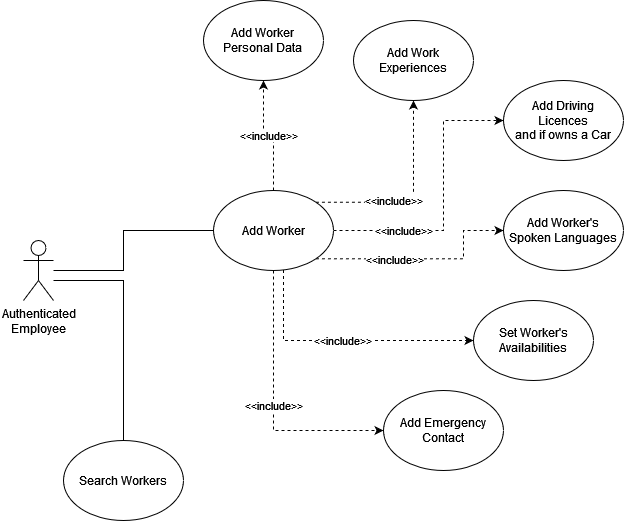
\includegraphics[width = 10 cm]{images/casiduso}
	% \caption{}
	\label{fig:casi d'uso}
\end{figure}

\subsection{Inserimento nuovo lavoratore}
I dipendenti dell’agenzia per poter effettuare l’inserimento e la gestione delle anagrafiche dei lavoratori è necessario che siano autenticati al sistema. \\

%\newgeometry{
%	a4paper,
	% total={170mm,257mm},
	% left=20mm,
	% top=10mm,
%}

\fbox{%
	\parbox{\textwidth}{%
		\textbf{Attori:} Dipendente dell’agenzia \\
		\textbf{Precondizioni:} Il dipendente deve essere autenticato. \\ 
		\textbf{Passi:}
		\begin{enumerate}
			\item Il dipendente accede al sistema
			\item Il dipendente è introdotto all’interfaccia di base
			\item Il dipendente compila il form con i dati anagrafici e il contatto di emergenza o modifica un form di un lavoratore esistente 
			\item Il dipendente inserisce il nuovo lavoratore o salva le modifiche del lavoratore modificato
		\end{enumerate}
		\textbf{Postcondizioni:}  Il lavoratore viene aggiunto dal database
	}%
}

\begin{figure}[h!]
	\centering
	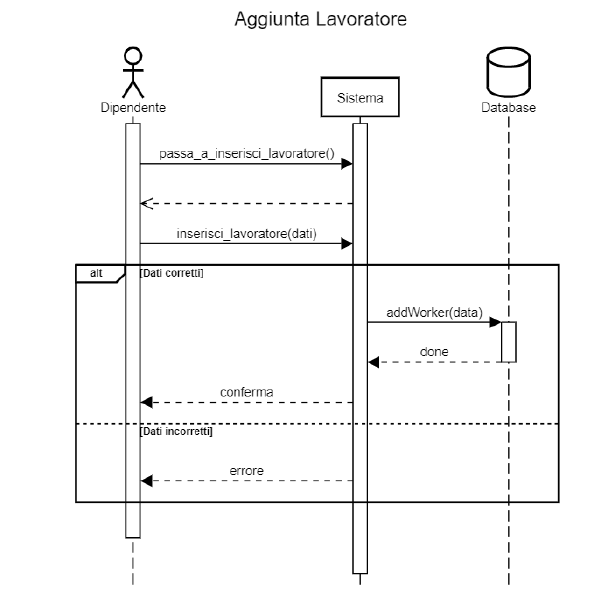
\includegraphics[width = 10 cm]{images/aggiunta}
	% \caption{}
	\label{fig:Inserimento lavoratore}
\end{figure}

\newpage\subsection{Effettuare ricerche}
I dipendenti dell’agenzia per poter effettuare delle ricerche complesse è necessario che siano autenticati al sistema. \\
La ricerca può avvenire mediante una barra di testo tramite l’inserimento di nome e cognome.
\'E inoltre possibile filtrare ulteriormente i risultati in base a: lingue parlate, mansioni effettuate, periodo e comuni di disponibilità,
patenti di guida e disponibilità di auto propria. Tutti questi filtri possono inoltre essere applicati in modalità “AND” oppure “OR”. \\

\fbox{%
	\parbox{\textwidth}{%
		\textbf{Attori:} Dipendente dell’agenzia \\
		\textbf{Precondizioni:} Il dipendente deve essere autenticato. \\ 
		\textbf{Passi:}
		\begin{enumerate}
			\item Il dipendente accede al sistema
			\item Il dipendente è introdotto all’interfaccia di base
			\item Il dipendente visualizza la lista dei lavoratori
			\item Il dipendente filtra la lista dei lavoratori
		\end{enumerate}
	}%
}

\begin{figure}[h!]
	\centering
	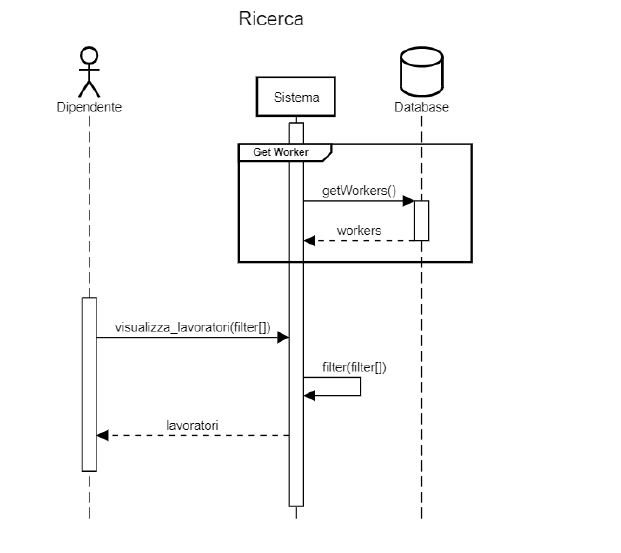
\includegraphics[width = 10 cm]{images/ricerca}
	% \caption{}
	\label{fig:Ricerca lavoratore}
\end{figure}

\newpage
\subsection{Cancellazione lavoratore}
I dipendenti dell’agenzia per poter cancellare un lavoratore è necessario che siano autenticati al sistema. \\
La cancellazione avviene tramite un pulsante dedicato per ogni lavoratore. \\

\fbox{%
	\parbox{\textwidth}{%
		\textbf{Attori:} Dipendente dell’agenzia \\
		\textbf{Precondizioni:} Il dipendente deve essere autenticato. \\ 
		\textbf{Passi:}
		\begin{enumerate}
			\item Il dipendente accede al sistema
			\item Il dipendente è introdotto all’interfaccia di base
			\item Il dipendente visualizza la lista dei lavoratori
			\item Il dipendente trova il lavoratore da eliminare
			\item Il dipendente elimina il lavoratore tramite apposito pulsante
		\end{enumerate}
		\textbf{Postcondizioni:}  Il lavoratore viene eliminato dal database
	}%
}

\newpage
\section{Diagrammi di attività}
\subsection{Autenticazione}
I dipendenti dell’agenzia per poter poter utilizzare il software è necessario che siano autenticati al sistema.

\begin{figure}[H]
	\centering
	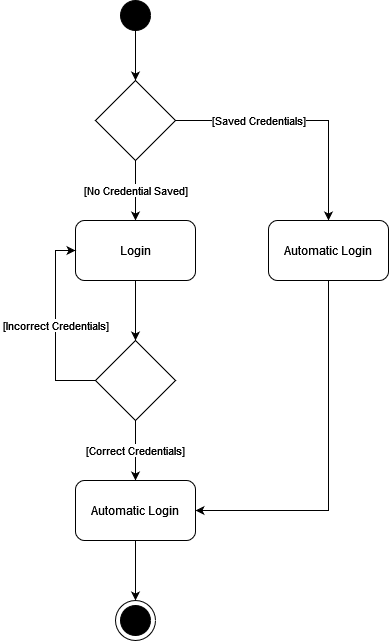
\includegraphics[width = 10 cm]{images/logincredenziali.png}
	% \caption{}
	\label{fig:login credenziali}
\end{figure}

\newpage
\subsection{Gestione delle anagrafiche}

\begin{figure}[H]
	\centering
	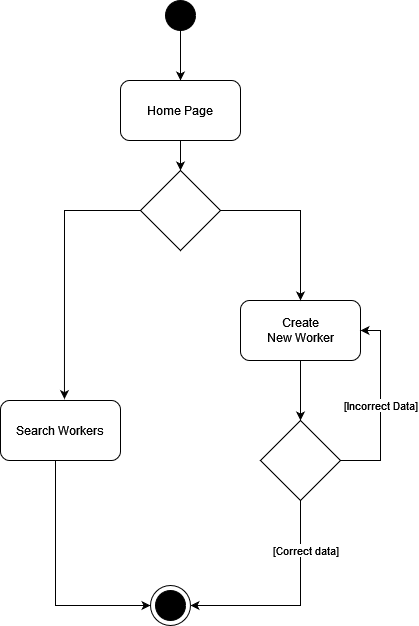
\includegraphics[width = 10 cm]{images/attivitadipendenti.png}
	% \caption{}
	\label{fig:attività dipendenti}
\end{figure}

Nota: i seguenti diagrammi catturano una singola attività di un utente rispetto al sistema. Non è stata rappresentata nel diagramma la possibilità di ripetere più volte la stessa operazione, in sequenza, senza chiudere il software. Questo per semplici ragioni di chiarezza e leggerezza; si considerano quindi le singole attività d’interazione

\newpage

\section{Note sul processo di sviluppo}
Il processo di sviluppo è stato basato su un approccio Agile e Incrementale, con l'obiettivo di mantenere una solida base di lavoro. 
L'implementazione delle funzionalità non ha seguito un piano rigido, ma è stato scelto, ad ogni incremento, cosa fosse prioritario integrare
ai fini di ridurre le tempistiche di sviluppo. Dopo ogni modifica significativa, è stata eseguita una rapida attività di test. La fase di analisi 
dei requisiti è stata completata prima dello sviluppo, che ha comportato la creazione di Use-Cases, diagrammi di attività e progettazione architetturale.


\newpage

\section{Design Pattern BLoC}
Il design pattern scelto è \textit{\texttt{BLoC}}, un design pattern creato da Google con lo scopo di separare la Business Logic dal Presentation Layer 
e permettere allo sviluppatore di riutilizzare il codice in modo efficiente. Per semplificare il tutto, viene messa a disposizione una libreria 
per Dart chiamata \textit{\texttt{flutter\_bloc}} che aiuta lo sviluppatore nell'implementazione del design pattern.

Nell'architettura Bloc, la Business Logic è centralizzata all'interno della classe blocco, mentre la visualizzazione è gestita da widget che ascoltano 
gli stati del blocco e reagiscono di conseguenza. Questo semplifica la separazione della logica di business dall'interfaccia utente e consente quindi 
di testare la logica di business in modo più efficiente. 

Questo pattern è particolarmente utile per le app di medie e grandi dimensioni, dove la gestione della Business Logic risulta complessa. 

BLoc Design Pattern si basa sul concetto di Programmazione Reattiva. La programmazione reattiva è un paradigma di programmazione che si concentra 
sulla gestione degli eventi e delle modifiche ai dati in tempo reale. Invece di eseguire il codice in modo sequenziale, la programmazione reattiva 
utilizza flussi di dati e eventi che possono essere trasmessi tra i diversi componenti dell'applicazione in modo asincrono. 

Il concetto di base è quello dello Stream. Uno stream è una sequenza di dati che possono essere trasmessi e/o ricevuti in modo asincrono,
anche da più componenti dell'applicazione.

Questo comporta che:
\begin{itemize}
	\item quando succede qualcosa in qualsiasi componente (un evento, una variabile modificata \ldots) viene inviata una notifica a uno Stream
	\item chi si trova in ascolto su quello Stream, verrà avvisato e potrà quindi intraprendere le azioni appropriate, qualunque sia la sua posizione all'interno dell'applicazione
\end{itemize}

Ogni componente (\textit{widget}) della User Interface ad ogni evento che lo riguarda dovrà semplicemente inviare una notifica dell'evento su uno Stream dedicato. 
Non dovrà preoccuparsi di chi userà quel dato, come o quando.

\newpage
\section{Architettura}
La libreria BLoC consente di separare l'applicazione in tre livelli:

\begin{description}
	\item [$\bullet$ Presentation Layer] (interfaccia utente) \hfill \\
	La responsabilità del Presentation Layer è quella di generare l'interfaccia utente tenendo conto dello stato di uno o più Bloc. 
	Inoltre deve gestire l'input dell'utente e i vari eventi del ciclo di vita dell'applicazione.
	\item [$\bullet$ Business Logic Layer] (bloc) \hfill \\
	La responsabilità del Business Logic Layer è rispondere agli eventi ricevuti dal Presentation con la generazione di nuovi stati. 
	Questo strato può appoggiarsi a uno o più Repository per recuperare i dati necessari alla creazione del nuovo stato.
	\item [$\bullet$ Data Layer] \hfill \\
	La responsabilità del Data Layer è quella di recuperare/manipolare i dati da una o più fonti.
	\begin{description}
		\item [$\cdot$ Repository] \hfill \\ 
		È un wrapper attorno a uno o più Data Provider. Si occupa di fornire dei dati ben formattati e facilmente utilizzabili al Bloc
		\item [$\cdot$ Data Provider] \hfill \\
		Recupera i “dati grezzi” direttamente dalla sorgente (il database).
	\end{description}
\end{description}

\begin{figure}[H]
	\centering
	
\includegraphics[width = 12 cm]{images/bloc_architecture.png}
	\label{fig:Architettura BLoC}
\end{figure}

\newpage
\newgeometry{
	bottom = 0mm,
}
\section{Backend}
La realizzazione del Backend è stata affidata a Appwrite, un backend-as-a-service open source e self-hosted che semplifica lo sviluppo
di app con una suite di SDK e API. Appwrite fornisce vari servizi tra cui autenticazione e database.

\subsection{Autenticazione}
Appwrite offre delle API dedicate per gestire l’autenticazione dell’app. Tramite la SDK è possibile accedere a delle funzioni per 
registrare e autenticare gli utenti e gestirne la sessione.

\subsection{Database}
Appwrite offre un database basato su documenti di facile utilizzo. Dietro le quinte si tratta di un database NoSQL basato su MariaDB. 
Il database si compone di:

\begin{description}
	\item[$\bullet$ Collection:]un gruppo di documenti. Ogni collezione ha degli attributi che definiscono la struttura del documento e le sue 
	autorizzazioni per la lettura e la scrittura.
	\item[$\bullet$ Document:]un oggetto JSON strutturato di chiavi e valori, appartenente a una Collection.
\end{description}

Le \textbf{Collection}, i \textbf{Document}, gli \textbf{Attributi} e i \textbf{Permessi} possono essere facilmente gestiti dalla console di Appwrite. \\
La SDK di Appwrite mette a disposizione dei metodi per caricare, aggiornare, eliminare i \textbf{Documents} delle rispettive \textbf{Collections}.

\begin{figure}[H]
	\centering
	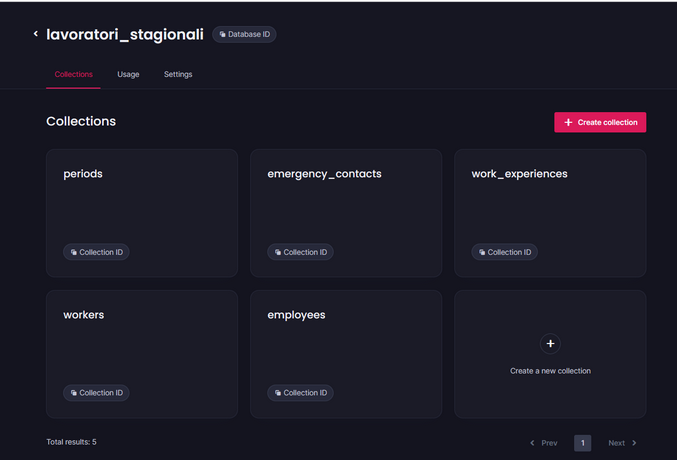
\includegraphics[width = 15 cm]{images/appwrite.png}
	\label{fig:interfaccia Appwrite}
\end{figure}








\end{document}

